\section{Hauptseite}\label{sec:main-page}

Die Hauptseite erreicht man, wenn man fulib.org das erste Mal öffnet.
Dabei präsentiert sich der sogenannte Vier-Panel-Editor, welcher in Abbildung~\ref{fig:four-pane-editor} dargestellt wird.
Diese zeigt oben links den Scenario-Editor sowie die darüberliegende Toolbar.
Oben rechts gibt es ein Fenster für den generierten Java-Code, welches auch die Konsolenausgabe des Compilers enthält.
Darüber zeigt eine Statusleiste, ob das Kompilieren und Ausführen erfolgreich war und wenn nicht, welches Tool fehlgeschlagen ist.
Im unteren Teil werden links das Klassendiagramm und rechts die Objektdiagramme dargestellt.

\begin{figure}
    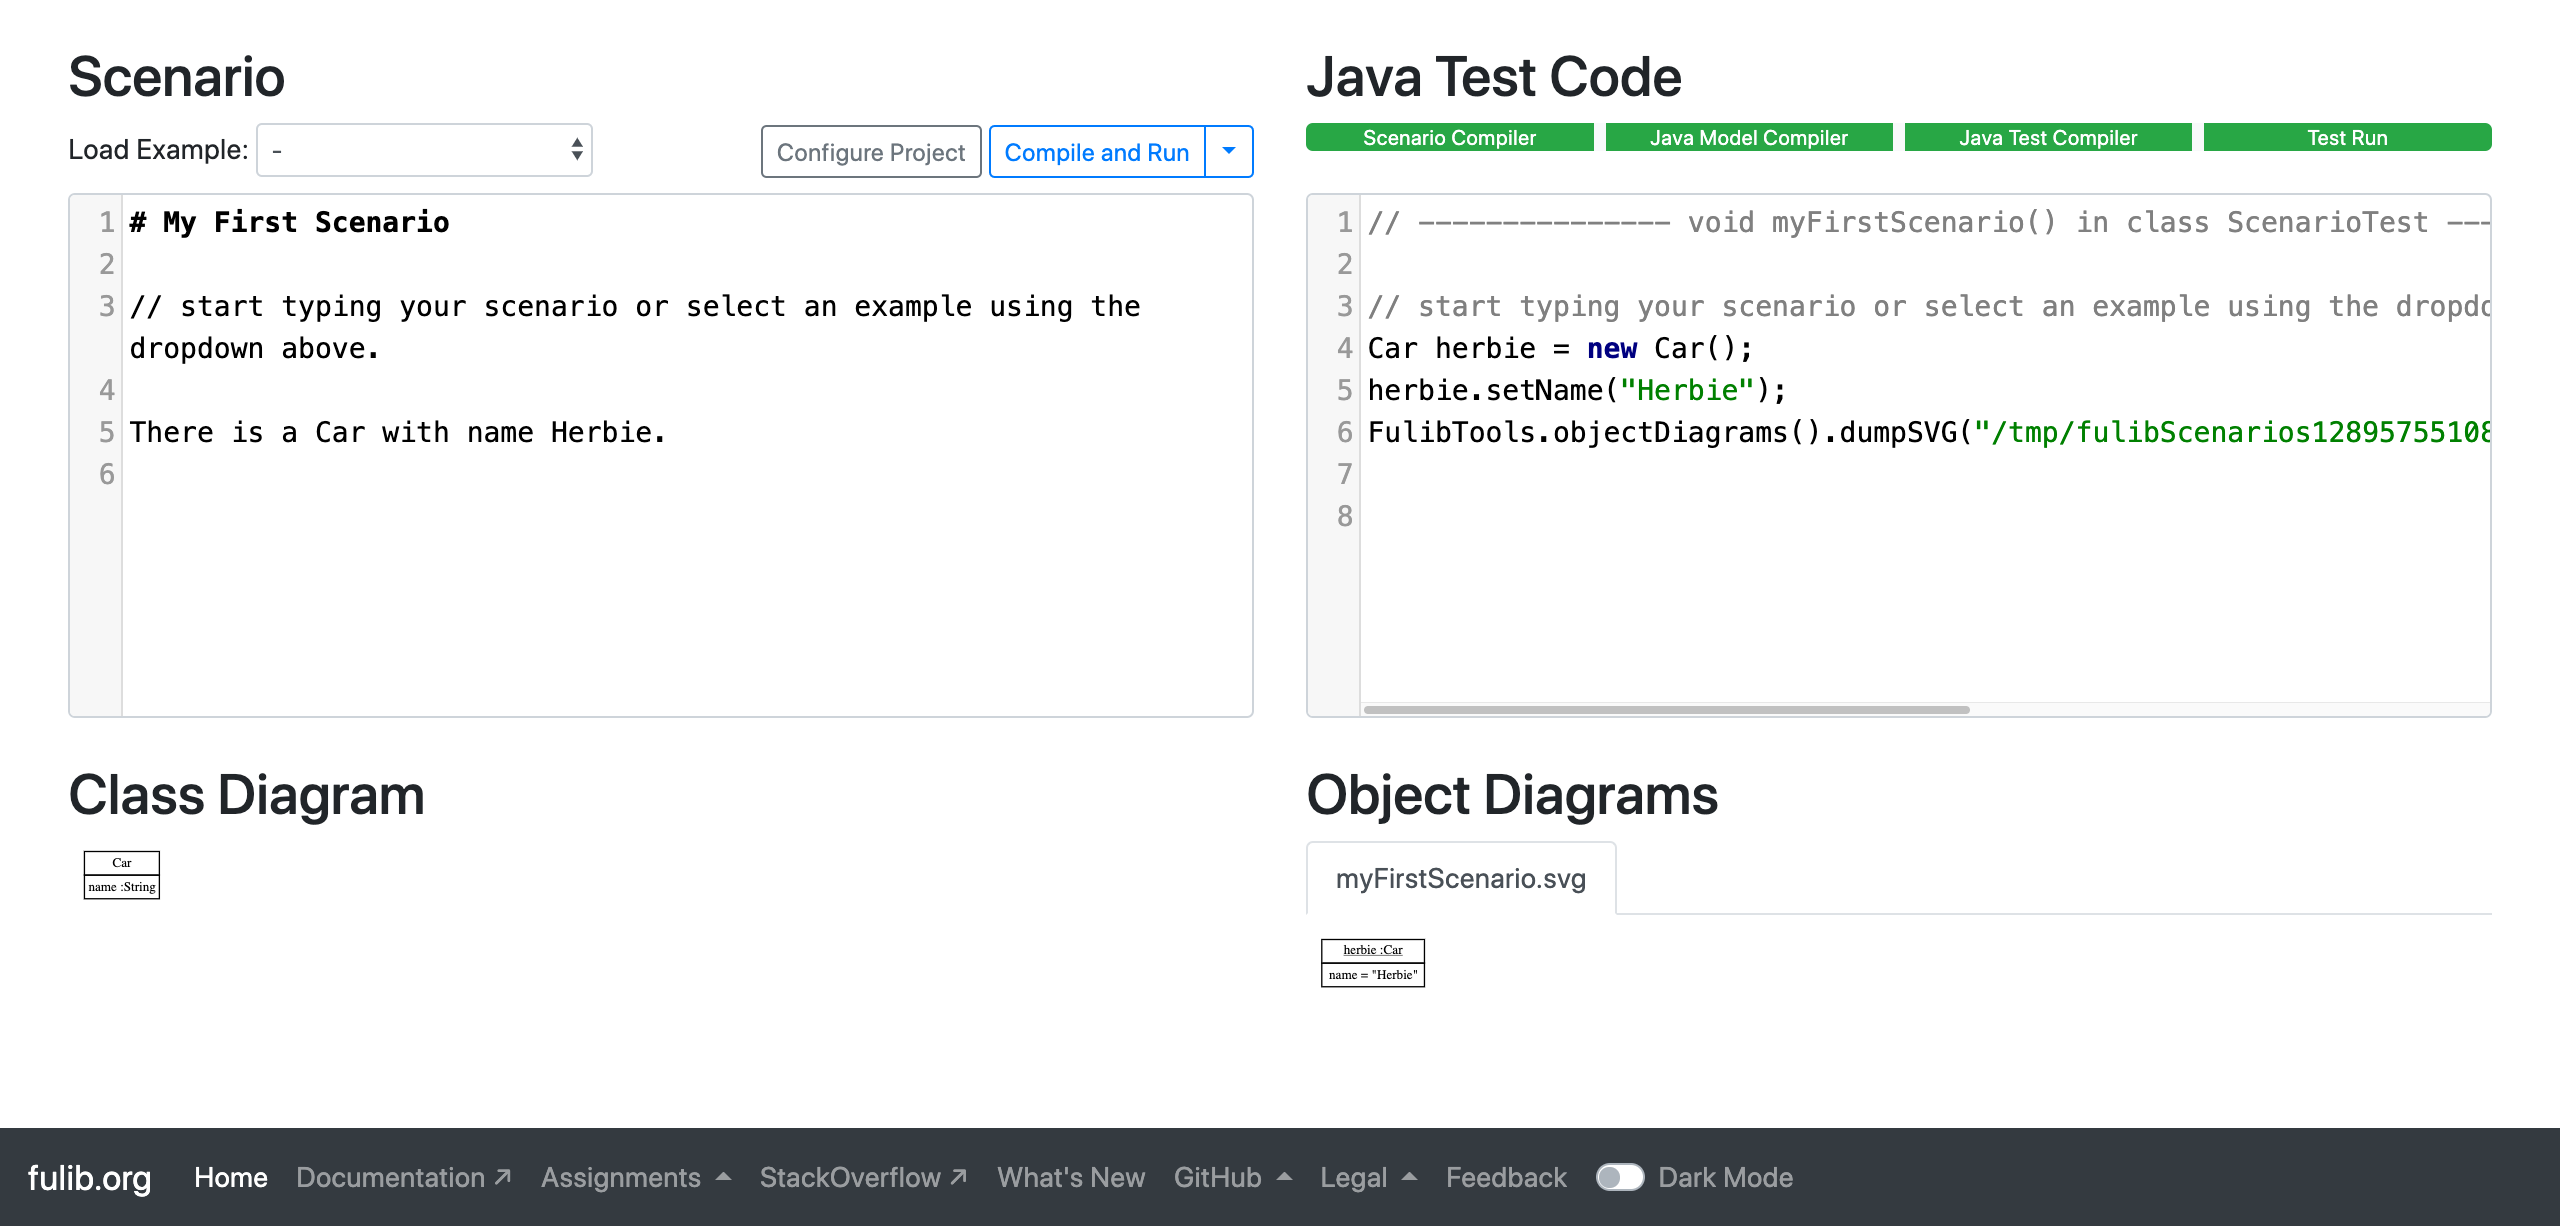
\includegraphics[width=\textwidth]{chapter/fulib.org/img/four-pane-editor.png}
    \caption{Der Vier-Panel-Editor auf der Hauptseite von fulib.org}
    \label{fig:four-pane-editor}
\end{figure}

Am unteren Rand der Seite befindet sich stets der Footer.
Dieser enthält Links zur Navigation innerhalb der Webseite und zu externen Referenzen.
Unter ``Legal'' befinden sich Links zu Impressum und Datenschutzrichtlinien sowie die Einstellungen zur Datenspeicherung.
``What's New'' zeigt den Versionsverlauf der Webseite und anderer Fulib-Bibliotheken und -Tools.
Die Schaltfläche ``Feedback'' öffnet ein Fenster, in dem Probleme gemeldet, Änderungen vorgeschlagen und Hilfe angefordert werden können.
Auch der Schalter zum Wechseln in den Nachtmodus (eng.: Dark Mode) ist stets im Footer sichtbar.

\subsection{Scenario-Editor}\label{subsec:scenario-editor}

Die wichtigste Funktion der Hauptseite ist der Scenario-Editor.
Gibt man darin ein Scenario ein und klickt auf ``Compile and Run'', wird daraus Java-Code generiert und dessen Tests mit JUnit ausgeführt.
Das dabei entstehende Klassendiagramm sowie Objektdiagramme werden dann in den entsprechenden Bereichen angezeigt.
Um das sofortige Feedback zu erleichtern, wird das Scenario immer automatisch ausgeführt, wenn es länger als eine Sekunde unverändert bleibt.
Somit muss nicht manuell auf ``Compile and Run'' geklickt werden.
Alternativ kann die automatische Ausführung im Dropdown-Menü neben dem ``Compile and Run''-Button deaktiviert werden.
Manuell lässt sie sich dann weiterhin durch Klick oder Verwenden der Tastenkürzel (\code{Strg/Cmd-S}, \code{Strg/Cmd-Enter}) auslösen.

Im Fenster für den Java-Code werden die Rümpfe sämtlicher Methoden angezeigt, die im Scenario verwendet wurden.
Davon ausgenommen sind aufgrund ihrer Trivialität Getter und Setter sowie diverse standardmäßig generierte Methoden.
Die Ausgabe des Scenario- und Java-Compilers sowie der JUnit-Testausführung werden ebenfalls in diesem Fenster angezeigt.
Dabei sind die Meldungen des Scenario-Compilers besonders relevant, da diese auf Fehler im Scenario hinweisen.

Objektdiagramme werden unter Tabs angeordnet.
Dies vermeidet Unübersichtlichkeit bei der Verwendung von vielen Diagramm-Sätzen im Scenario.
Die einzelnen Darstellungen lassen sich dann getrennt voneinander betrachten.

\subsection{Tutorials}\label{subsec:tutorials}

Über dem Scenario-Editor befindet sich ein Auswahlfeld für vordefinierte Tutorials.
Wählt man eines davon aus, wird dessen Scenario-Text in den Editor übernommen und sofort ausgeführt.
Die Tutorials sind in Kategorien angeordnet und bauen in ihrer Reihenfolge aufeinander auf.
Somit werden die behandelten Sprachkonzepte zunehmend komplexer.

In den Tutorial-Scenarios ist beschreibender Text mit \code{//}-Kommentaren realisiert.
Diese bewirken, dass der Text auch im Java-Code auftaucht, was die Zuordnung von Sätzen zu Anweisungen vereinfacht.
Durch Abschnitte erfolgt eine visuelle Trennung von unabhängigen Teil-Scenarios.

Am Ende jedes Tutorials gibt es Links zu entsprechenden Abschnitten in der Dokumentation, die detaillierte Informationen zu den verwendeten Sprachkonzepten enthalten.
Darunter sind auch formale Definitionen der Syntax in Form einer Grammatik sowie Erklärungen zu häufigen Problemfällen zu finden.

Die von Tutorials stammenden Scenarios können frei verändert werden.
Dadurch können die Sprachkonzepte direkt ausprobiert werden.
Lädt man das entsprechende Tutorial erneut, wird wieder der vordefinierte Scenario-Text verwendet und die Änderungen verworfen.

\subsection{Projektexport}\label{subsec:project-export}

Neben dem ``Compile and Run''-Button befindet sich der Button ``Configure Project''.
Damit lässt sich das Fenster zur Projektkonfiguration öffnen, welches in Abbildung~\ref{fig:project-config} zu sehen ist.
In diesem werden Einstellungen zum Projekt durchgeführt, zu dem das Scenario später gehören soll.
Genauer lassen sich dessen Name und Version sowie Paket und Dateiname des Scenarios einstellen.
Diese werden wie der Scenario-Text im Browser gespeichert, damit sie beim erneuten Aufrufen der Seite bestehen bleiben.
Eingestellte Werte haben nur geringen Einfluss auf die Funktionalität der Webseite selbst, jedoch sind sie beim Herunterladen eines Projekts von Relevanz.
Dies ist mit einem Button im unteren Teil des Fensters möglich.
Klickt man auf diesen, wird das Scenario zusammen mit einigen Konfigurationsdateien in einem Zip-Archiv verpackt und heruntergeladen.
Bei den Konfigurationsdateien handelt es sich um jene, die das Build-Tool Gradle~\cite{gradle} benötigt.
Dieses ist zuständig für Kompilierung, Dependency-Management, Test-Ausführung und andere Build-Aufgaben in Java-Projekten.
Das Projekt ist voreingestellt, um den Scenario-Compiler in den Build-Prozess zu integrieren.

\begin{figure}
    \centering
    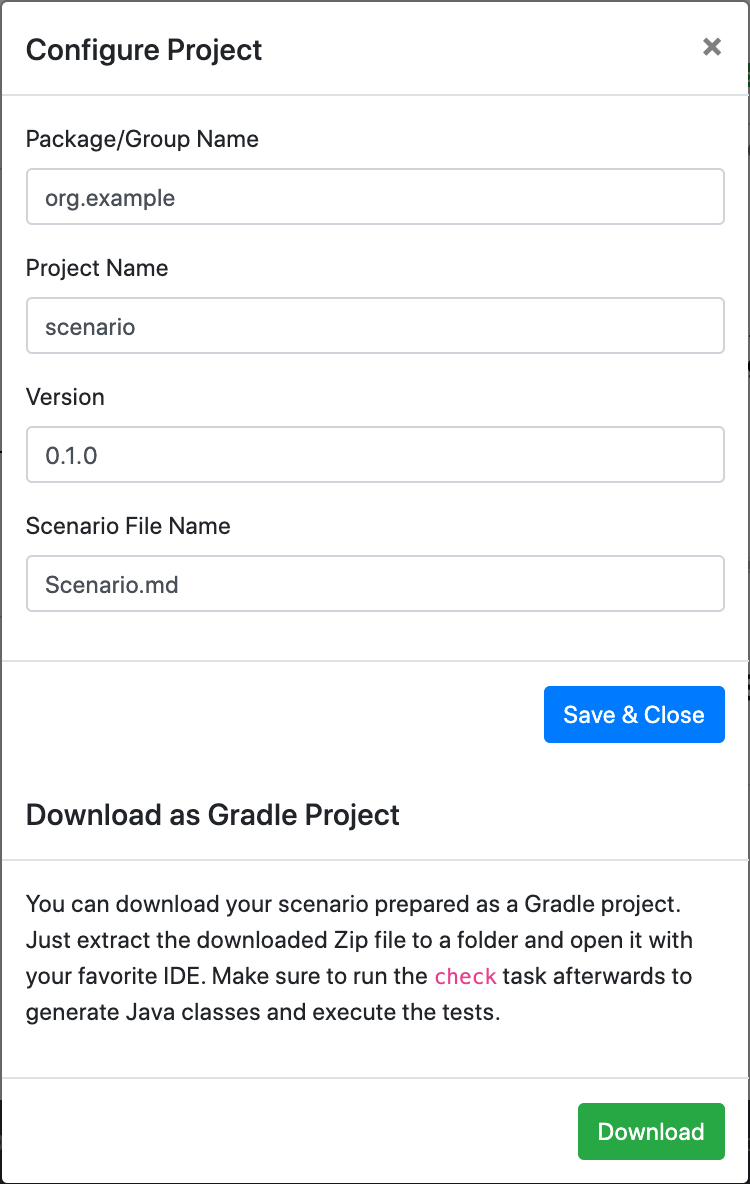
\includegraphics[width=0.5\textwidth]{chapter/fulib.org/img/project-config.png}
    \caption{Projektkonfiguration}
    \label{fig:project-config}
\end{figure}

Entpackt man das heruntergeladene Archiv, erhält man einen fertigen Projektordner.
Dieser kann in einer IDE mit Gradle-Unterstützung wie IntelliJ geöffnet werden.
Führt man daraufhin den \code{check}-Task mit Gradle aus (Kommandozeile: \code{./gradlew check} im Projektordner), wird das zuvor auf fulib.org geschriebene Scenario kompiliert und generierte Java-Dateien in den entsprechenden Ordnern unter \code{src/} abgelegt.
Außerdem bewirkt \code{check} die Ausführung von generierten Tests.
Abbildung~\ref{fig:project-downloaded} zeigt, wie ein Projektordner in IntelliJ unmittelbar nach dem Download und nach Ausführen des \code{check}-Tasks aussehen kann.
Ändert man die Scenario-Datei und führt den Task erneut aus, wird auch der Java-Code angepasst.

\begin{figure}
    \centering
    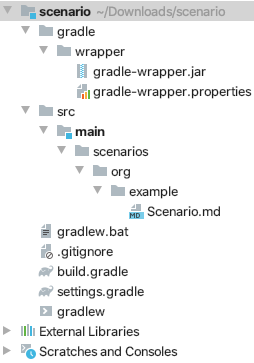
\includegraphics[width=0.25\textwidth]{chapter/fulib.org/img/project-downloaded.png}
    \hspace{0.05\textwidth}
    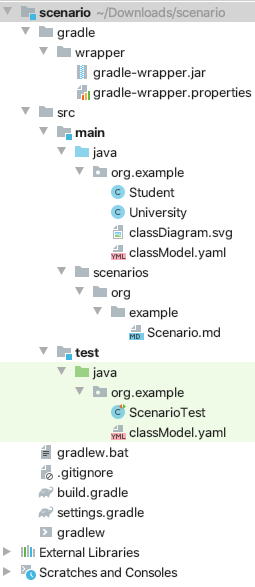
\includegraphics[width=0.25\textwidth]{chapter/fulib.org/img/project-post-check.png}
    \caption{Heruntergeladenes Projekt in IntelliJ vor und nach Ausführen des \code{check}-Tasks}
    \label{fig:project-downloaded}
\end{figure}

Der Projektexport ist vor allem dann relevant, wenn das Scenario zu groß wird, um im Editor übersichtlich zu sein.
In einem eigenständigen Projekt können dann mehrere Scenario-Dateien angelegt werden, auf die das ursprüngliche Scenario aufgeteilt werden kann.
Ein weiterer Vorteil ist, dass der generierte Java-Code vollständig einsehbar und anpassbar ist.
Es bietet sich an, das Projekt unter Versionskontrolle wie Git zu stellen.
Im Projektarchiv ist eine voreingestellte \code{.gitignore}-Datei enthalten, um dessen Einrichtung zu erleichtern.

\subsection{Sicht der Studenten}\label{subsec:students-view}

Im Wintersemester 2019/20 haben Studierende der Uni Kassel die Scenario-Sprache, die fulib.org-Seite und die damit erstellten Projekte verwendet.
Dies geschah im Modul ``Programmieren und Modellieren'', das im Bachelor zum dritten Fachsemester gehört.
Es wurden zunächst die Webseite und die Scenarios in der Vorlesung erklärt.
In zwei Hausaufgaben wurde dann der Einsatz beider Tools bewertet.
Die erste davon befasste sich mit der Modellierung eines einfachen Datenmodells und dem anschließenden Projektexport.
Ziel der zweiten Hausaufgabe war es, mit Scenarios ein GUI-Mockup zu entwickeln.
Dafür kam das FulibMockups-Tool zum Einsatz, welches parallel zu FulibScenarios entwickelt wurde und darauf aufbaut.
Es erlaubt das Modellieren von Benutzeroberflächen als Objektstrukturen, aus denen HTML-Seiten sowohl statisch als auch in Form von Klickprototypen generiert werden.
Beide Hausaufgaben sind in ihrer Bewertung im Vergleich zu anderen Aufgabenblättern im Modul überdurchschnittlich gut ausgefallen.

Am Ende des Semesters konnten die Studierenden bei einer Umfrage ihr Feedback zur Vorlesung hinterlassen.
Diese enthielt auch einige Fragen zu fulib.org, FulibScenarios und FulibMockups.
Dabei konnten fünf Aspekte mit einer Note von 1 bis 6 bewertet werden.
Tabelle~\ref{tab:survey-results} zeigt die Durchschnittsnoten der Aspekte.
Insgesamt haben 28 von 55 zum Zeitpunkt der Umfrage an der Vorlesung teilnehmenden Studierenden ihre Antworten eingereicht.
Die genaue Verteilung der Noten sowie sonstige Umfrageergebnisse sind in Anhang~\ref{sec:survey-results} zu finden.

\begin{table}
    \caption{Durchschnittliche Bewertung der Teilbereiche in der Vorlesungsumfrage PM WS19/20}
    \label{tab:survey-results}
    \centering
    \begin{tabular}{rl}
        \toprule
        2,7 & Scenario-Sprache \\
        2,3 & Beispielscenarios \\
        2,8 & Fehlermeldungen \\
        2,8 & Mockups \\
        2,4 & Webseite \\
        \bottomrule
    \end{tabular}
\end{table}

Eine weitere Frage befasste sich mit zukünftigen Features in Form einer Mehrfach-Auswahl.
Dabei waren insbesondere jene genannt, die den Online-Editor betreffen.
Die meisten Studierenden (24 von 28) haben sich Syntaxhighlighting gewünscht, gefolgt von der Hervorhebung von Fehlern und Warnungen im Code (20 von 28).
Auch zur Auswahl standen Autovervollständigung (18 von 28) und die Möglichkeit, mehrere Scenarios gleichzeitig in Tabs zu öffnen (10 von 28).

Durch ein Freitext-Feld gab es die Möglichkeit, allgemeines Feedback zu hinterlassen.
Darin wurde mehrfach die fehlende Dokumentation kritisiert.
Diese war zum Zeitpunkt der Verwendung durch die Studierenden unvollständig, weshalb sie nicht öffentlich zugänglich war.
Inzwischen wurde diese wesentlich erweitert und ist nun auf fulib.org verlinkt.

Auch wurde die Verständlichkeit der Fehlermeldungen kritisiert.
Wie im folgenden Abschnitt erläutert wird, wurden auch diese erweitert, um die Lösungssuche zu erleichtern.
Die Beispielscenarios wurden angepasst, um verständlicher zu sein.
Zusätzlich wurden sie mit Links zur Dokumentation ausgestattet.
Gleichzeitig kann auch in der Dokumentation auf Beispiele verlinkt werden, um die darin enthaltene Beschreibung von Sprachkonzepten interaktiv zu ergänzen.

Das FulibMockups-Projekt befindet sich derzeit im einem frühem Stadium der Entwicklung.
In Zukunft soll es insbesondere in der Typsicherheit und Ausdrucksstärke verbessert werden.
Das Hinzufügen von Autovervollständigung kann dessen Gebrauch auch vereinfachen.

\subsection{Datensammlung}\label{subsec:data-collection}

Öffnet man fulib.org das erste Mal, erscheint das Fenster mit den Datenschutz-Einstellungen, das in Abbildung~\ref{fig:privacy} gezeigt ist.
Darin kann ausgewählt werden, ob man lokale (d.h. im Browser) oder serverseitige Datenspeicherung erlauben möchte.

\begin{figure}
    \centering
    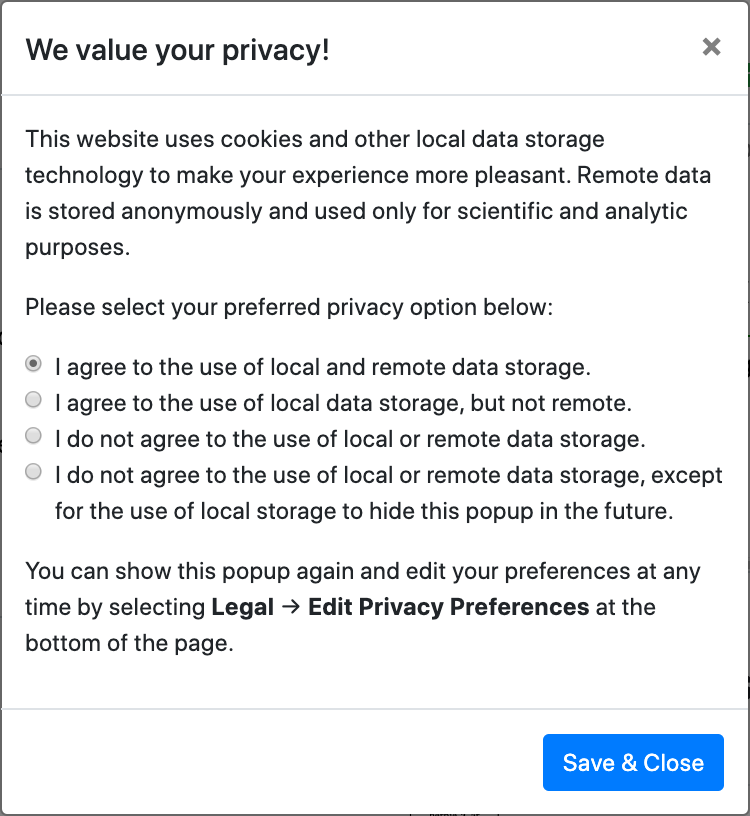
\includegraphics[width=0.5\textwidth]{chapter/fulib.org/img/privacy.png}
    \caption{Datenschutzeinstellungen}
    \label{fig:privacy}
\end{figure}

Zu lokale Daten zählen auf der Hauptseite der Scenario-Text sowie die Projekteinstellungen.
Erlaubt man die lokale Speicherung nicht, werden diese nach erneutem Laden der Seite auf Standardwerte zurückgesetzt.
Außerdem wird die Auswahl der Datenschutzeinstellung selbst lokal gespeichert.
Ist dies nicht erlaubt, öffnet sich das Einstellungsfenster bei jedem Besuch von fulib.org automatisch.
Für datenschutzbewusste Benutzer, die dies als Störung empfinden, gibt es daher die vierte Option, welche die lokale Datenspeicherung lediglich zum Verstecken des Fensters nutzt.

Die serverseitige Datenspeicherung umfasst sämtliche ``Compile and Run''-Anfragen, die an den Server gesendet werden.
Der Server speichert dann die vollständige Anfrage (d.h. Scenario-Text und Projektkonfiguration) und die vollständige Antwort.
Letztere enthält Compiler-Ausgaben, Methodenrümpfe und Diagramme.
Weiterhin werden IP-Adresse und User-Agent\footnote{Dabei handelt es sich um einen HTTP-Header, der die Browser-Version sowie meist das Betriebssystem identifiziert.} der Anfragen protokolliert, was deren progressive Anordnung erlaubt.
Dies ermöglicht beispielsweise die Analyse des Zeitaufwands, der für das Lesen und Verstehen der Beispielscenarios benötigt wird.

Während der Vorlesung ``Programmieren und Modellieren'' im Wintersemester 2019/20 konnte serverseitig eine Vielzahl von Daten gesammelt werden.
Zum Zeitpunkt der Messung am 16.\ Februar 2020, 18:00, wurden seit 1.\ Oktober 2019 etwa 5100 Anfragen gespeichert.
Aufgrund der veränderlichen Natur von IP-Adressen und User-Agent-Zeichenketten kann nicht auf die Anzahl der unterschiedlichen Benutzer geschlossen werden.
Außerdem ist nicht bekannt, wie viele Nutzer die serverseitigen Datenspeicherung abgelehnt haben.
Dennoch haben die gesammelten Daten bereits hohen Wert gezeigt.
Da die Fehlermeldung des Scenario-Compilers IDs wie \code{[variable.redeclaration]} enthalten, kann in dem Datensatz leicht nach ihnen gesucht werden.
Von den oben genannten 5100 Anfragen enthielten 847 mindestens eine Fehler- oder Warnmeldung.
Insgesamt belief sich die Zahl der gefundenen Meldungen auf 1949.
Tabelle~\ref{tab:error-counts} stellt diese dar.

\begin{table}
    \caption{Zusammengefasste Anzahl der Fehlermeldungen nach ID}
    \label{tab:error-counts}
    \centering
    \begin{tabular}{rl}
        \toprule
        21	& \code{[remove.source.type]} \\
        29	& \code{[property.unresolved]} \\
        33	& \code{[write.target.list]} \\
        34	& \code{[association.reverse.conflict]} \\
        39	& \code{[descriptor.multi.indefinite.deprecated]} (Warnung) \\
        65	& \code{[add.target.type]} \\
        86	& \code{[attribute.reverse.name]} \\
        177	& \code{[descriptor.indefinite.deprecated]} (Warnung) \\
        254	& \code{[property.redeclaration.conflict]} \\
        283	& \code{[has.subject.primitive]} \\
        288	& \code{[property.declaration.first]} (Hinweis) \\
        298	& \code{[variable.redeclaration]} \\
        298	& \code{[variable.declaration.first]} (Hinweis) \\
        44  & sonstige Fehler \\
        \midrule
        1949 & Gesamt (inkl.\ Hinweise) \\
        1363 & Fehler- und Warnmeldungen \\
        1147 & Fehlermeldungen \\
        \bottomrule
    \end{tabular}
\end{table}

Zu den häufigsten Meldungen zählen hier \code{[property.declaration.first]} und \code{[variable. declaration.first]}. % manual line break
Dabei handelt es sich weder um Fehler, noch um Warnungen.
Diese Meldungen sind Hinweise und treten in Kombination mit den Fehlern \code{[association.reverse.conflict]} und \code{[property.redeclaration.conflict]} bzw. \code{[variable.redeclaration]} auf.
Die Hinweise deuten auf vorherige Stellen im Scenario und erleichtern dadurch das Verständnis und die Lösung der Probleme.
Warnmeldungen sind hier ausschließlich Deprecations, welche bei Verwendungen von Syntax auftreten, die in Zukunft nicht mehr unterstützt werden soll.

Die Statistik, welche Fehler am meisten auftraten, hatte besonderen Wert bei der Verbesserung der Fehlermeldungen.
So konnte priorisiert werden, welche Änderungen die größte Wirkung erzielen können.
Im Verlauf dieser Arbeit ist eine Hinweismeldung hinzugekommen, welche auf eventuelle Tippfehler bei Werten und Attribut- und Assoziationsnamen verweist.
Diese findet bei zehn in der Tabelle gezeigten Fehlerarten Anwendung (vier davon unter ``sonstige''), welche insgesamt 775 Mal aufgetreten sind.
Dies entspricht einer Verbesserung von etwa zwei dritteln aller Fehlermeldungen.
